\chapter{Background}
\label{chap:background}

In this chapter...

\section{Event correlation}

\subsection{Scenario-based Correlation}
\iffalse
https://dl.acm.org/doi/pdf/10.1145/1501434.1501479
\fi
\subsection{Statistical Correlation}
\subsection{Temporal Correlation}
\subsection{Hybrid approaches}

\iffalse
\cite{Ludovic_2004} to propose a fully functional intrusion detection system based on event and alert correlations. Among the several approaches available in the literature, we chose to implement a language driven signature based correlation. Uses FSM to implement the multi-pattern rule matching detection algorithm.
\fi
\subsection{Finite State Machine Based}
% What are finite state machines?
A finite-state machine, a system is abstracted into mathematical model which can have exactly one of a finite number of states at a time. A finite-state machine has a fixed set of possible states, a set of inputs that change the state, and a set of possible outputs \cite{keller_2001}.
The next state of a finite-state machine is based on the current state that the machine is in, and the input that change the state.
There are generally considered to be two kinds of finite-state machines, deterministic finite-state machines and non-deterministic finite-state machines. In a deterministic finite-state machine, every state has only one transition per input, as opposed to the non-deterministic state machine, where an input can lead to none, one or many transitions for a given state. Since the deterministic finite-state machine is a more strict version of the non-deterministic finite-state machine, that leads to that by definition, a deterministic finite-state machine is also a non-deterministic finite-state machine.
For example, assuming that we have the following three events in order:
\begin{enumerate}
    \item the process '$word.exe$' started
    \item the process '$googlechrome.exe$' started
    \item The process '$powershell.exe$' started
\end{enumerate}
If we want to trigger an alert when we see the $word.exe$ process is created, and then the $powershell.exe$ process afterwards, we can design a simple non-deterministic state machine like the one in figure \ref{fig:finite-state-machine}. When applying the above-mentioned events to this finite state-machine, event number one will move our state from $s_0$ to $s_1$. Event number two will not do any transitions and change the state (one of the benefits of using a non-deterministic state machine). When event number three occurs, the state machine transitions from $s_1$ to $s_2$, and our accepting state is reached, which fulfills the state machine and we can create an alarm.
\begin{figure}[ht]
\centering
\begin{tikzpicture}[->,>=stealth',shorten >=1pt,auto,node distance=4cm,
                    thick,main node/.style={circle,draw,font=\sffamily\Large\bfseries}]
  \node[initial,state] (p1) {$s_0$};
  \node[state] (p2) [right of=p1] {$s_1$};
  \node[state,accepting] (p3) [right of=p2] {$s_2$};

  \path[every node/.style={font=\sffamily\small}]
    (p1)
        edge node {'word.exe' started} (p2)
    (p2)
        edge node {'powershell.exe' started} (p3)
    ;
\end{tikzpicture}
\caption{Example of non-deterministic finite-state machine}
\label{fig:finite-state-machine}
\end{figure}
One of the benefits of the finite-state model is that it is possible to specify if the order of the events are important or not. If the event order is not of interested, a finite-state machine as shown in Figure \ref{fig:finite-state-machine-2} can represent the same case as seen in Figure \ref{fig:finite-state-machine}.
\begin{figure}[ht]
\centering
\begin{tikzpicture}[->,>=stealth',shorten >=1pt,auto,node distance=1.5cm,
                    thick,main node/.style={circle,draw,font=\sffamily\Large\bfseries}]
  \node[initial,state] (s0) {$s_0$};
  \node[] (middle) [right of=s0] {};
  \node[state] (s1) [above of=middle] {$s_1$};
  \node[state] (s2) [below of=middle] {$s_2$};
  \node[state,accepting] (s3) [right of=middle] {$s_3$};

  \path[every node/.style={font=\sffamily\small}]
    (s0)
        edge node {'word.exe' started} (s1)
        edge node [swap] {'powershell.exe' started} (s2)
    (s1)
        edge node {'powershell.exe' started} (s3)
    (s2)
        edge node [swap] {'word.exe' started} (s3)
    ;
\end{tikzpicture}
\caption{Example of non-deterministic finite-state machine}
\label{fig:finite-state-machine-2}
\end{figure}

An approach to use finite-state machines for event correlation has been shown in \cite{Bouloutas_1992} where the authors use observed events that are generated by the monitored process to feed into the modelled finite-state machine that represent the monitored process. If an event arrives that leads to an invalid state in the model, an error is produced.

One of the main drawback with the finite-state machine is the missing notion of time. As shown in Figure \ref{fig:finite-state-machine-2} we can take into account order of events, but a finite-state machine does not separate on the time difference between events that are streamed into the model.

\subsection{Rule Based Event Correlation}
\subsection{Case Based Reasoning}

In case based reasoning, a previously experienced problem and its solution is called a case. As explained in \cite{aamodt_1994}, case based reasoning is based on the assumption that we can find a solution for a new problem by finding past cases that are similar, and then reusing the solution to solve the new problem. The reasoning is then further enforced by adding the problem and the solution to the case library for future use.
As stated in \cite{slade_1991}, case-based reasoning is similar to how humans approach new problems by assimilating past experiences and adapting them to new situations.

Figure \ref{fig:case-based-reasoning-cycle} describes the cycle used in case-based reasoning from a high-level perspective.
Under each step in the cycle there are multiple tasks that may be necessary to conduct before continuing on with the cycle. For instance, the "Retrieve" step might need to identify which features of the problem to search the Case Library for.
\begin{figure}[ht]
\centering
%\tikzstyle{startstop} = [rectangle, rounded corners, minimum width=3cm, minimum height=1cm,text centered, draw=black, fill=red!30]
\begin{tikzpicture}[->,>=stealth',shorten >=1pt,auto,node distance=2cm,
                    thick,main node/.style={circle,draw,font=\sffamily\Large\bfseries},
                    problemm/.style={circle, text centered, draw=black, fill=red!30},
                    stepp/.style={rectangle, minimum width=3cm, minimum height=1cm,text centered, draw=black, fill=orange!30},
                    libraryy/.style={rectangle, rounded corners, minimum width=3cm, minimum height=1cm,text centered, draw=black, fill=green!30}]
  \node (Problem) [problemm] {Problem};
  \node (Retrieve) [stepp, below of=Problem] {Retrieve};
  \node (Reuse) [stepp, below of=Retrieve] {Reuse};
  \node (Revise) [stepp, below of=Reuse] {Revise};
  \node (Retain) [stepp, right of=Revise, xshift=3cm] {Retain};
  \node (CaseLibrary) [libraryy, right of=Retrieve, xshift=3cm] {Case Library};
  
  \path[every node/.style={font=\sffamily\small}]
    (Problem)
        edge node {} (Retrieve)
    (Retrieve)
        edge node {} (Reuse)
    (Reuse)
        edge node {Copy or Adapt} (Revise)
    (Revise)
        edge node {Evaluate} (Retain)
    (Retain)
        edge node {} (CaseLibrary)
    (CaseLibrary)
        edge node {} (Retrieve)
    ;
\end{tikzpicture}
\caption{Case-based reasoning cycle}
\label{fig:case-based-reasoning-cycle}
\end{figure}\\
A example where this might be useful is in a Security Operations Center (SOC). A SOC receives a high number of alerts that have to be handled by an analyst to analyse and propose a response to the alert. The response can vary from simply suppressing the alert as a false-positive, sending an e-mail to the client to alert them, or escalating the alarm to the Incident Response team. Case based reasoning can then be applied to new alerts by first retrieving the most similar alerts previously handled. The information stored in the previous case can then be used to handle the analysis or solution to an alert. The analyst will then revise the proposed solution, and retain the parts that might be useful for resolving similar future alerts. This follows the case based reasoning cycle proposed in \cite{aamodt_1994}.
The retrieval step is difficult because we need to find similar cases that offer solutions that are relevant. Cases may contain attributes that are irrelevant, which might not be clear to the automated retrieval process. \cite{lewis_1993} and \cite{davies_1987} propose creating "determination rules" or "determinators" that are either compound attributes or a pointer to which attributes to look at in the case.
Additionally, adaptation of the old solutions to the new problem is a difficult task. While manual specification of the solution in the "Revise" step is possible and somewhat required, too much emphasis on manual intervention or adjustments will defeat the purpose of case-based reasoning. This is why according to \cite{leake_1996} many case-based reasoning systems have adapted the cycle from Retrieve-Reuse-Revise-Retain to a much shorter Retrieve-Propose cycle that completely eliminates the adaptation.

In \cite{schwartz_2002}, the authors used the intrusion detection system Snort as a basis for a new case-based reasoning IDS that uses the Snort rule base as a case library. Snort rules may in general be too specific and fail to detect certain kind of intrusions, but with the case-based reasoning approach, the retrieval step in the cycle will take care of this by finding cases (rules) that are applicable to the network packet even though the vanilla rule would not create an alert on that packet.
In \cite{Kapetanakis_2014}, the authors argue that with the digital traces left by an attacker, it is possible to build a profile for that attacker which can be used to assist in future attacks to identify which attacker is attacking. In \cite{han_2016} the authors implemented a system called "WHAP" which uses case-based reasoning to compare cyber attacks against websites. WHAP builds on a large database of website defacements, which are custom webpages left on the victim server by the attacker to claim credit for a website hack. The system is then able to take new hacked websites as input, and output similar previous cases where it is likely that the website has been hacked by the same attacker. This can be useful for attribution and forensic investigations.

\subsection{Model Based Reasoning}
Model-based reasoning is a expert system where the target is to create a model that can be used to predict the outcome of input event or faults in the system. The idea of modelling the structure and behavior of a system has its roots in \cite{davies_1987} where their work explore the use of such models in troubleshooting digital electronics.  There are no fixed way for how a system can or should be modelled. The model itself can be created as a logical formalization using pure mathematics, or as a simulated system using for example a game engine. As the authors of \cite{Dodig-Crnkovic2017} highlight, there is an increased interest in automating the creation of the model of a system. This is based on the fact that creating and keeping a model consistent with the system it is supposed to model, is hard.
In \cite{jakobson_1993} model-based reasoning is discussed for alarm correlation for fault management in telecommunications networks.


\iffalse


The managed system is modeled
with respect to its event emission behavior (event model). The programmed knowledge somehow
defines events to be related under some temporal or sequential constraints

A description of the 


structure, the topology, connectivity of components
behaviour description,
a set of principles to guide the troubleshooting \cite{davies_1987}

\fi

In the paper \cite{poll_2003}, a figure similar to \ref{fig:model-based-reasoning-example} is shown. It outlines the process for checking if a modelled system is consistent with the real world system it is supposed to replicate.

\begin{figure}[ht]
\centering
\begin{tikzpicture}[->,>=stealth',shorten >=1pt,auto,node distance=2cm,thick
                    ]
  \node (PhysicalSystem) [xshift=-1cm] {Physical system};
  \node (Model) [xshift=1cm, right of=PhysicalSystem] {Model of system};
  \path (PhysicalSystem) -- (Model) coordinate[midway] (aux);
  
  \node (Actions) [below of= aux] {Actions};
  
  \node (Observed) [below of= Actions,xshift=-2cm] {Observed behavior};
  \node (Predicted) [below of= Actions,xshift=2cm] {Predicted behavior};
  \path (Observed) -- (Predicted) coordinate[midway] (aux2);
  
  \node (Discrepancy) [below of= aux2] {Discrepancy?};
  
  \node (no) [below of= Discrepancy,xshift=-2cm,text width=3.5cm] {Model is consistent with system};
  \node (yes) [below of= Discrepancy,xshift=2cm,text width=3.5cm] {Search over model\\to explain discrepancy};
  
  \path[every node/.style={font=\sffamily\small}]
    (PhysicalSystem)
        edge node {} (Actions)
    (Model)
        edge node {} (Actions)
    (Actions)
        edge node {} (Observed)
        edge node {} (Predicted)
    (Observed)
        edge node {} (Discrepancy)
    (Predicted)
        edge node {} (Discrepancy)
    (Discrepancy)
        edge node [swap] {No} (no)
        edge node {Yes} (yes)
    ;
\end{tikzpicture}
\caption{Illustration of model-based reasoning}
\label{fig:model-based-reasoning-example}
\end{figure}
As stated in \cite{sethi_2001}, one of the primary drawbacks of model-based reasoning is the requirement to have a well structured system to model and to keep that model updated. Systems that contain fluctuating objects like for example computer networks or network services are not trivial to represent in a formal model. More applicable areas might include hardware diagnostics like shown in \cite{davies_1987}, or other areas where it is possible to model a more static target system, like for example automobile diagnostics. Furthermore, \cite{Venkatasubramanian_2003} discuss that various implementations of model-based reasoning is quite computational complex, depending on number of objects in the model and their various inputs and outputs.

\subsection{Codebook Based Event Correlation}
\label{sub:codebook-based-event-correlation}

\begin{figure}[ht]
\centering
\begin{tikzpicture}[->,>=stealth',shorten >=1pt,auto,node distance=3cm,
                    thick,main node/.style={circle,draw,font=\sffamily\Large\bfseries}]
  \node[main node] (p1) {$p^1$};
  \node[main node] (p2) [right of=p1] {$p^2$};
  \node[main node] (p3) [right of=p2] {$p^3$};
  \node[main node] (e1) [below left of=p1] {$e^1$};
  \node[main node] (e2) [right of=e1] {$e^2$};
  \node[main node] (e3) [right of=e2] {$e^3$};
  \node[main node] (e4) [right of=e3] {$e^4$};

  \path[every node/.style={font=\sffamily\small}]
    (p1)
        edge node {} (e1)
        edge node {} (e2)
        edge node {} (e3)
    (p2)
        edge node {} (e2)
        edge node {} (e3)
        edge node {} (e4)
    (p3)
        edge node {} (e1)
        edge node {} (e2)
        edge node {} (e4)
    ;
\end{tikzpicture}
\caption{Example causality graph used for codebook based event correlation}
\label{fig:causality-graph-codebook}
\end{figure}

In \cite{yemini_1996}, the authors propose that the events caused by problems can be modelled as seen in figure \ref{fig:causality-graph-codebook} where the directed edges of the graph describe the causality of an event. $p^x$ denotes a problem, and $e^x$ denotes an event. To utilize the codebook, each problem node in the graph is converted into a binary vector can be created to describe its relation to the events on the graph. This is known as a "code". The binary vector contains bits that corresponds to each event in the graph. If a bit is set to a $1$, it indicates that the given problem causes the event that the bit corresponds to. A bit of $0$ indicates that it does not cause the event. These codes then go into the codebook. If we convert the graph in figure \ref{fig:causality-graph-codebook} into a codebook, it will look like table \ref{tab:correlation-matrix}. The graph and codebook needs to be sufficiently large to be able to identify all the problems. If the codebook is too small, it may omit events that are of interest to us. If the codebook is too large, it may contain events that are unnecessarily redundant. One way to approach the problem with codebooks that are too large, is to do what the authors in \cite{yemini_1996} calls "codebook reduction". Codebook reduction is the process of removing events that are "universal" for all problems. In the figure \ref{fig:causality-graph-codebook} and the corresponding table \ref{tab:correlation-matrix} we can see that event $e^2$ is a common event for all the problems. Because of this redundancy, it can be remove to simplify the codebook as show in table \ref{tab:correlation-matrix-reduced}. Further work has been done to enhance the efficiency of the codebook. \cite{gupta_1999} proposes a two step preprocessing algorithm that ensures mathematical provable codebooks and eliminates events that are unable to distinguish between problems.

When new events occur, the events are converted into a new binary vector. This vector is then compared with the codes in the codebook, and the code that is the most similar is chosen as a means to identify the problem. A simple approach for comparing the binary vectors could be a 1-to-1 comparison to see if the new binary vector exactly matches any of the codes in the codebook, but \cite{yemini_1996} propose to instead use Hamming distance to calculate the closest match. Using Hamming distance has several benefits, first of all it increases the tolerance for noise or lost events, secondly instead of choosing a single best candidate problem, we can defined a radius that will give us a codebook subset containing possible codes within the given Hamming distance radius.
Because of the novel preprocessing down to binary vectors, codebook-based correlation is faster than other rule-based event correlation techniques. One of the more time-consuming tasks with regard to codebook-based event correlation is the creation of the problems and their mapping to symptom events. The most likely way to produce these codebooks will be as an expert system where a person with deep knowledge about the events in the system are able to map symptoms to problems. In addition, the process of selecting which events might be symptoms of a problem is similar to feature selection in the machine learning landscape. Feature selection is the process of selecting a subset of features that can be used in model construction, which is similar to how the codebook is generated.

One of the biggest limitations regarding codebook based event correlation is that there is no built-in way to handle time. When a problem has been identified based on a number of symptoms, there is no time window applied, and there is no notion of event order. Furthermore the events do not contain any properties, and would require significant extending to take into account e.g. source hostname, username.

\begin{table}[ht]
\centering
\begin{tabular}{l|llll}
 & $e^1$ & $e^2$ & $e^3$ & $e^4$ \\ \hline
$p^1$ & 1 & 1 & 1 & 0 \\
$p^2$ & 0 & 1 & 1 & 1 \\
$p^3$ & 1 & 1 & 0 & 1
\end{tabular}
\caption{Codebook correlation matrix}
\label{tab:correlation-matrix}
\end{table}

\begin{table}[ht]
\centering
\begin{tabular}{l|lll}
 & $e^1$ & $e^3$ & $e^4$ \\ \hline
$p^1$ & 1 & 1 & 0 \\
$p^2$ & 0 & 1 & 1 \\
$p^3$ & 1 & 0 & 1
\end{tabular}
\caption{Reduced codebook correlation matrix}
\label{tab:correlation-matrix-reduced}
\end{table}

\subsection{Voting approaches}
\subsection{Explicit Fault-localization}
\subsection{Dependency Graphs}


\begin{figure}[ht]
\centering
\begin{tikzpicture}[->,>=stealth',shorten >=1pt,auto,node distance=3cm,
                    thick,main node/.style={circle,draw,font=\sffamily\Large\bfseries}]
  \node[main node] (a) {a};
  \node[main node,fill=blue] (b) [right of=a] {b};
  \node[main node,fill=blue] (c) [right of=b] {c};
  \node[main node,fill=blue] (d) [below left of=a] {d};
  \node[main node] (e) [right of=d] {e};
  \node[main node] (f) [right of=e] {f};
  \node[main node] (g) [right of=f] {g};
  \node[main node] (h) [below left of=d] {h};
  \node[main node,fill=red] (i) [right of=h] {i};
  \node[main node] (j) [right of=i] {j};
  \node[main node] (k) [right of=j] {k};
  \node[main node] (l) [right of=k] {l};

  \path[every node/.style={font=\sffamily\small}]
    (a)
        edge node {} (e)
    (b)
        edge node {} (e)
    (c)
        edge node {} (f)
    (d)
        edge node {} (h)
        edge node {} (i)
    (e)
        edge node {} (j)
    (f)
        edge node {} (j)
        edge node {} (k)
    (g)
        edge node {} (k)
        edge node {} (l)
    (j)
        edge node {} (i)
    ;
\end{tikzpicture}
\caption{Example dependency graph}
\label{fig:dependency-graph}
\end{figure}

Similar to the dependency graph used in \ref{sub:codebook-based-event-correlation}, \cite{Gruschke_1998} suggests that a dependency graph can contain enough information to be used for event correlation, while also being simple to automatically generate. The dependency graph is a directed graph that maps the relationship managed objects. These objects can be hosts in a network, dependencies in a micro-service architecture, and so forth.
In figure \ref{fig:dependency-graph} we have mapped a series of objects as an example. Events are mapped to their corresponding object in the graph (colored in blue, object b, c and d). Then we walk the graph from those objects. As explained in \cite{Gruschke_1998}, when we optimally find one object node that are common for all the given events, we have most likely found the responsible node. In the example this is marked as red, object i.
\cite{Gruschke_1998} further outlines that the quality of the root-cause detection can be measured by the depth and length we need to walk the graph at. Objects that are further away from the initial object are less likely to be the root cause, and vica versa.
One of the main drawbacks of dependency graph based correlation is the fact that it does not handle multiple, non-related problems very well. \cite{Gruschke_1998} assumes that only one problem occurs at a time. If multiple problems occur that are not related or affect each other, finding the root-case may prove to be impossible, or select the wrong root-cause object.
Assumes the events are for a single fault. Meaning it will not be able to handle detecting multiple failing nodes.
As with the codebook-based event correlation we discussed in \ref{sub:codebook-based-event-correlation}, dependency graphs also lack the notion of time. Additionally the dependency graph is not taking advantage of attributes on the nodes to further enhance the graph.

\subsection{Bayesian Network Based Event Correlation}

Bayesian networks are one of the most widely used graphical models for representing and reasoning about the probabilistic causal relationships between variables\cite{Kavousi_2014}. Bayesian networks are usually represented by directed acyclic graphs. Directed acyclic graphs are finite directed graphs that contain no direct cycles. This means that there is no way to start from a given node, and via the directed edges return back to the same node. Each node in the network represents a variable of interest and the edges describe the relations between these variables.
The Bayesian network is split up into two parts. First there is the graphical model of the network which shows the nodes and the edges that connect them. Secondly, there is the conditional probability tables associated with each node. The table consist of the probabilities that a node is in a given state given the state of its parent nodes.



Both \cite{Kavousi_2014} and \cite{Qin_2004} utilize Bayesian networks to create "Bayesian attack graphs" (BAG) which are models that use Bayesian networks to depict the security attack scenarios in a system.

As a simple experiment using a Bayesian Network for detection, we have the directed acyclic graph as shown in Figure \ref{fig:simple-directed-acyclic-graph}. The nodes are a bit like the ones represented in Codebook-based correlation \ref{sub:codebook-based-event-correlation} where the nodes $B$ and $C$ represent two symptom events that are analyzed by the system, these can be events from an IDS, host machine logs, web logs, et cetera. The node $A$ represent a problem node and is not connected to any specific events. The purpose of this Bayesian network, is to answer the following question: What is the probability that, when we observe the two events $B$ and $C$, we have a problem $A$?

To calculate this, we first need the the conditional probability tables, which are given in Table \ref{tab:probabability-tables}.

\begin{figure}[ht]
\centering
\begin{tikzpicture}[->,>=stealth',shorten >=1pt,auto,node distance=1cm,
                    thick,main node/.style={circle,draw,font=\sffamily\Large\bfseries}]
  \node[main node] (a) {$A$};
  \node[main node] (b) [below of=a,xshift=-2cm] {$B$};
  \node[main node] (c) [below of=a,xshift=2cm] {$C$};

  \path[every node/.style={font=\sffamily\small}]
    (a)
        edge node {} (b)
        edge node {} (c)
    ;
\end{tikzpicture}
\caption{Simple example directed acyclic graph}
\label{fig:simple-directed-acyclic-graph}
\end{figure}

\begin{table}[ht]
\centering
\begin{tabular}{|l|l|}
\hline
$P(A = 0)$ & $P(A = 1)$ \\ \hline
$0.8$ & $0.2$ \\ \hline
\end{tabular}
\begin{tabular}{|l|l|l|}
\hline
$A$ & $P(B = 1|A)$ & $P(B = 0|A)$ \\ \hline
$1$ & $0.9$ & $0.1$ \\ \hline
$0$ & $0.05$ & $0.95$ \\ \hline
\end{tabular}
\centering
\begin{tabular}{|l|l|l|}
\hline
$A$ & $P(C = 1|A)$ & $P(C = 0|A)$ \\ \hline
$1$ & $0.95$ & $0.05$ \\ \hline
$0$ & $0.05$ & $0.95$ \\ \hline
\end{tabular}
\caption{Conditional probability tables}
\label{tab:probabability-tables}
\end{table}

We can then calculate the probability that $A$ has occurred, given that we have observed the events $B$ and $C$ by using Bayes' theorem.
\begin{align*}
    &P(A=1 | B=1, C=1)\\
    &=\frac{P(A=1)P(B=1,C=1|A=1)}{P(B=1,C=1)}\\
    &=\frac{P(A=1)P(B=1,A=1)P(C=1,A=1)}{P(A=1)P(B=1|A=1)P(C=1|A=1)+P(A=0)P(B=1|A=0)P(C=1|A=0)}\\
    &=\frac{0.2\cdot0.9\cdot0.95}{(0.2\cdot0.9\cdot0.95)+(0.8\cdot0.05\cdot0.05)}\\
    &\approx 0.9884
\end{align*}
In this case, we see that there is approximately a 99\% chance that the problem/alert $A$ has happened, by observing the arrival of the two events $B$ and $C$.


\subsection{Neural Network Approaches}
\subsection{Etc}



\section{Rule-based event correlation}
\label{sec:eventcorrelation}
\todo{Give an intro into the world of correlating events, why is it so valuable?}

\begin{itemize}
    \item Reduce alert-fatigue by generating high-fidelity alerts.
    \item Gather up smaller events that in and of them self are not worthy an alarm.
\end{itemize}

Rule-based event correlation software is historically known as a expert system. \cite{cronk_1988} defines an expert system as a "problem-solving software that embodies specialized knowledge in a narrow task domain to do work usually performed by a trained, skilled human.".

According to \cite{cronk_1988}, expert systems are organized around three levels; data, control and task knowledge. \todo{See figure 2 in paper. It should be incorporated in some way, as it pretty much defines how we have built MEC}.

Traditionally, creating the rules that goes into a knowledge base is in \cite{cronk_1988} defined as two-fold; first you have the subject-matter expert which has the expertise and knowledge about which events you are interested in creating correlations against, and secondly the knowledge engineer which is familiar with how the expert system works and how the rules has to be written to be understood by the system.
In more modern settings, usually the subject-matter expert is also able to write rules

What are some of the drawbacks of rule-based event correlation?

\begin{itemize}
    \item Doesn't learn or adapt
    \item Requires the subject-matter expert to define the rules, and the knowledge engineer to implement them
    \item Time-consuming to write and "push" rules into the system
    \item Requires testing and monitoring to make sure that:
    \begin{enumerate}
        \item the rule triggers on the intended events and
        \item the rule does not create tons of alerts that will flood the analysts handling the alerts
    \end{enumerate} 
    \item Maintenance of the rule repository is time-consuming
    \item Networks may differ, so it's not given that a rule that fits into one network, can automatically be used in another.
\end{itemize}

Regardless of all the drawbacks, we see a common trend that rule-based systems are the most common when it comes to network-based monitoring (see Suricata, Snort) as well as for log data in SIEMs like Splunk, ELK, OSSEC and OSSIM.


There exists several different types of software that makes it possible to correlate events in real-time based on log data.

Software based on event correlation commonly referenced in academia today is largely defunct or the source code is unavailable. 

\begin{itemize}
    \item Swatch and 2swatch - defunct, single-threaded. Last updated in 1997?
    \item logsurfer \cite{thompson_2017} written in C. Improves upon Swatch.
    \item Simple Event Correlator (SEC) is still being actively developed to this date. This is the software that is the most prominent in the literature that I have found. I will address that tool in its own separate section under \ref{sec:SEC}.
    \item Variable Temporal Event Correlator (VTEC) - Built custom for log monitoring and correlation at the company Advanced Micro Devices (AMD). Can not find source code. Feature distributed "workers" and a "variable server" that holds state. Written in Perl and the software uses Perl-based rules.
    \item Event Query Language (EQL). Part of Endgame/Elastic. Written in Python. Scales vertically, same as SEC. Implements a Abstract Syntax Tree for Windows Event Logs specifically.
    \item KSQL - Supports correlation based on time in a Kafka queue. Limited to Kafka as queuing technology.
    \item Splunk - One of the most popular Enterprise SIEM solutions. Supports writing "alerts" that allow time-based correlations.
\end{itemize}
There are several other correlation-based systems other than the ones mentioned above, but they employ some form of machine learning or statistical analysis instead of a rule-based approach. This is usually used for anomaly detection or "finding the unknown" in a dataset, which is not the focus of this thesis.

\subsection{Simple Event Correlator}
\label{sec:SEC}

In the research that I have found, SEC is the most commonly referenced and used software for event correlation across different syslog events. It is widely used, and has been deployed in several different sectors and industries (Finance, Telecom, IT security, Government, Retail, etc. \cite{vaarandi2005tools}) and utilized for several different purposes like fraud detection, insider-threat detection, system fault and availability and security events. SEC is quite versatile, as it is agnostic to the type of log event that it receives. SEC uses rules that are using Perl-style regular expressions for matching events and extracting data from the event itself using sub-expressions. The extracted data can then be used to correlate between other matching events.

However, even though SEC is popular and commonly used, there are several improvements that could be done. Some of the constraints include:
\begin{itemize}
    \item Heavily based on regular expressions for writing rules, which makes it both hard to analyze rules, modifying existing rules and writing new rules.
    \item Current version can only be scaled vertically. The context-state used for correlation is per-process only and therefore any and all correlation between events have to happen in the same process. It is possible to use SEC in a multi-process fashion to handle separate log types, but this removes the possibility to correlate between those log types. 
    \item Few open source rules and rule-sets. The analyst generally has to start from scratch writing their own rules
    \item Limited support for multi-line logs
    \item Windows Event Logs has to be converted to syslog
    \item Made generic, not specific for Windows Event Logs
\end{itemize}

\subsection{Event Query Language}
\label{sec:eql}

Part of Endgame/Elastic. Written in Python. Scales vertically, same as SEC. Implements a Abstract Syntax Tree for Windows Event Logs specifically.

Is parsed "after the fact".


\section{Windows Event Log}

Windows Event Log is a built-in capability in the Microsoft Windows operating systems. The different event log categories can be configured using Group Policy Objects in an enterprise. The total amount of logs generated on a system is huge, so configuration is necessary to remove noisy or uninteresting events.
There are events for "everything". \todo{Find some examples here}
Windows Event Logs are usually sent to a centralized location for storage and analysis, either using the built-in option called Windows Event Log Forwarding or using custom agents like Splunk Universal Forwarder, winlogbeat or nxlog to name a few.

\subsection{Sysmon}
Sysmon is an extension to the stock Windows Event Log and allows for a more powerful customization of what events go into the event log. Using a kernel driver, Sysmon is able to add support for a wider variety of interesting events. The table \ref{tab:sysmoneventtypes} is a list of each event type that Sysmon can generate.

\begin{table}[ht]
\begin{tabular}{l|l}
ID & Description \\ \hline
1 & Process creation \\
2 & A process changed a file creation time \\
3 & Network connection \\
4 & Sysmon service state changed \\
5 & Process terminated \\
6 & Driver loaded \\
7 & Image loaded \\
8 & CreateRemoteThread \\
9 & RawAccessRead \\
10 & ProcessAccess \\
11 & FileCreate \\
12 & RegistryEvent (Object create and delete) \\
13 & RegistryEvent (Value Set) \\
14 & RegistryEvent (Key and Value Rename) \\
15 & FileCreateStreamHash \\
17 & PipeEvent (Pipe Created) \\
18 & PipeEvent (Pipe Connected) \\
19 & WmiEvent (WmiEventFilter activity detected) \\
20 & WmiEvent (WmiEventConsumer activity detected) \\
21 & WmiEvent (WmiEventConsumerToFilter activity detected) \\
22 & DNSEvent (DNS query) \\
255 & Error
\end{tabular}
\caption{List of Sysmon event types}
\label{tab:sysmoneventtypes}
\end{table}

\section{MITRE Cyber Analytics Repository}
"The MITRE Cyber Analytics Repository (CAR) is a knowledge base of analytics developed by MITRE based on the MITRE ATT\&CK adversary model"

One of the CAR analytics is "CAR-2013-04-002: Quick execution of a series of suspicious commands". This analytic is based on the assumption that certain commands are frequently ran by malicious actors on a system, while regular users do not run them. CAR-2013-04-002 outlines several commands of interest:
\begin{multicols}{2}
\begin{itemize}
\item arp.exe
\item at.exe
\item attrib.exe
\item cscript.exe
\item dsquery.exe
\item hostname.exe
\item ipconfig.exe
\item mimikatz.exe
\item nbstat.exe
\item net.exe
\item netsh.exe
\item nslookup.exe
\item ping.exe
\item quser.exe
\item qwinsta.exe
\item reg.exe
\item runas.exe
\item sc.exe
\item schtasks.exe
\item ssh.exe
\item systeminfo.exe
\item taskkill.exe
\item telnet.exe
\item tracert.exe
\item wscript.exe
\item xcopy.exe
\end{itemize}
\end{multicols}
\url{https://car.mitre.org/analytics/CAR-2013-04-002/}



\section{Sigma}
\url{https://github.com/Neo23x0/sigma}

Sigma is an open standard for rules that are used to generically describe searches in log data. It is primarily used as a high-level rule that transcompile into SIEM queries like Splunk, ElasticSearch, QRadar, etc. The rules are written in YAML (Yet Another Markup Language), and are key-value based.
\\
The following example Sigma rule is a basic rule that detects running \lstinline{ipconfig}, \lstinline{arp} and \lstinline{echo} within a ten second timeframe, filtered by the \lstinline{MachineName} key in the event: \todo{We should add some examples of what an event actually looks like, to make it more obvious to the reader what we are talking about here}

\begin{lstlisting}[
    basicstyle=\small
]
title: Quick Execution of a Series of Suspicious Commands
id: 61ab5496-748e-4818-a92f-de78e20fe7aa
description: Detects multiple suspicious process in a limited timeframe
status: experimental
references:
    - https://car.mitre.org/wiki/CAR-2013-04-002
author: Martin Ingesen
modified: 2020/01/01
tags:
    - car.2013-04-002
logsource:
    category: process_creation
    product: windows
detection:
    selection:
        CommandLine:
            - ipconfig
            - arp
            - echo
    timeframe: 10s
    condition: selection | count() by MachineName > 3
falsepositives:
    - False positives depend on scripts and
    administrative tools used in the monitored environment
level: low
\end{lstlisting}
The format contains some required and some optional fields, and is extensible with our own custom fields.

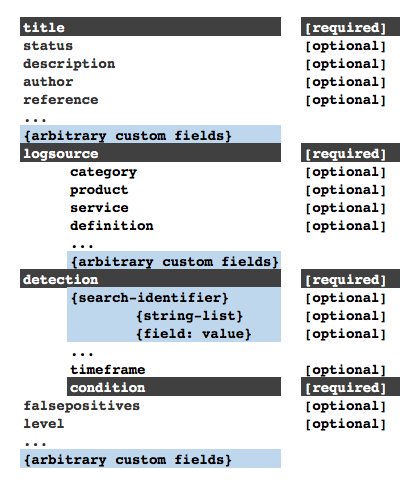
\includegraphics[scale=0.525]{figures/new-rule-format/Sigma_Schema.png}

Image source: \url{https://github.com/Neo23x0/sigma/wiki/Specification}